\section{Hardware}
Much of the hardware used in this project is not possible to simulate, due to
the nature of the integrated circuits involved.
However, one aspect that can be simulated is the analogue circuitry before the
codec.

\subsection{Signal Conditioning}
Models of the signal conditioning were created in OrCAD in order to check that
the break frequency and roll off were suitable.
The result of this modelling can be seen in figure \ref{fig:sigcondmodel}

\begin{figure}[H]
	\centering
	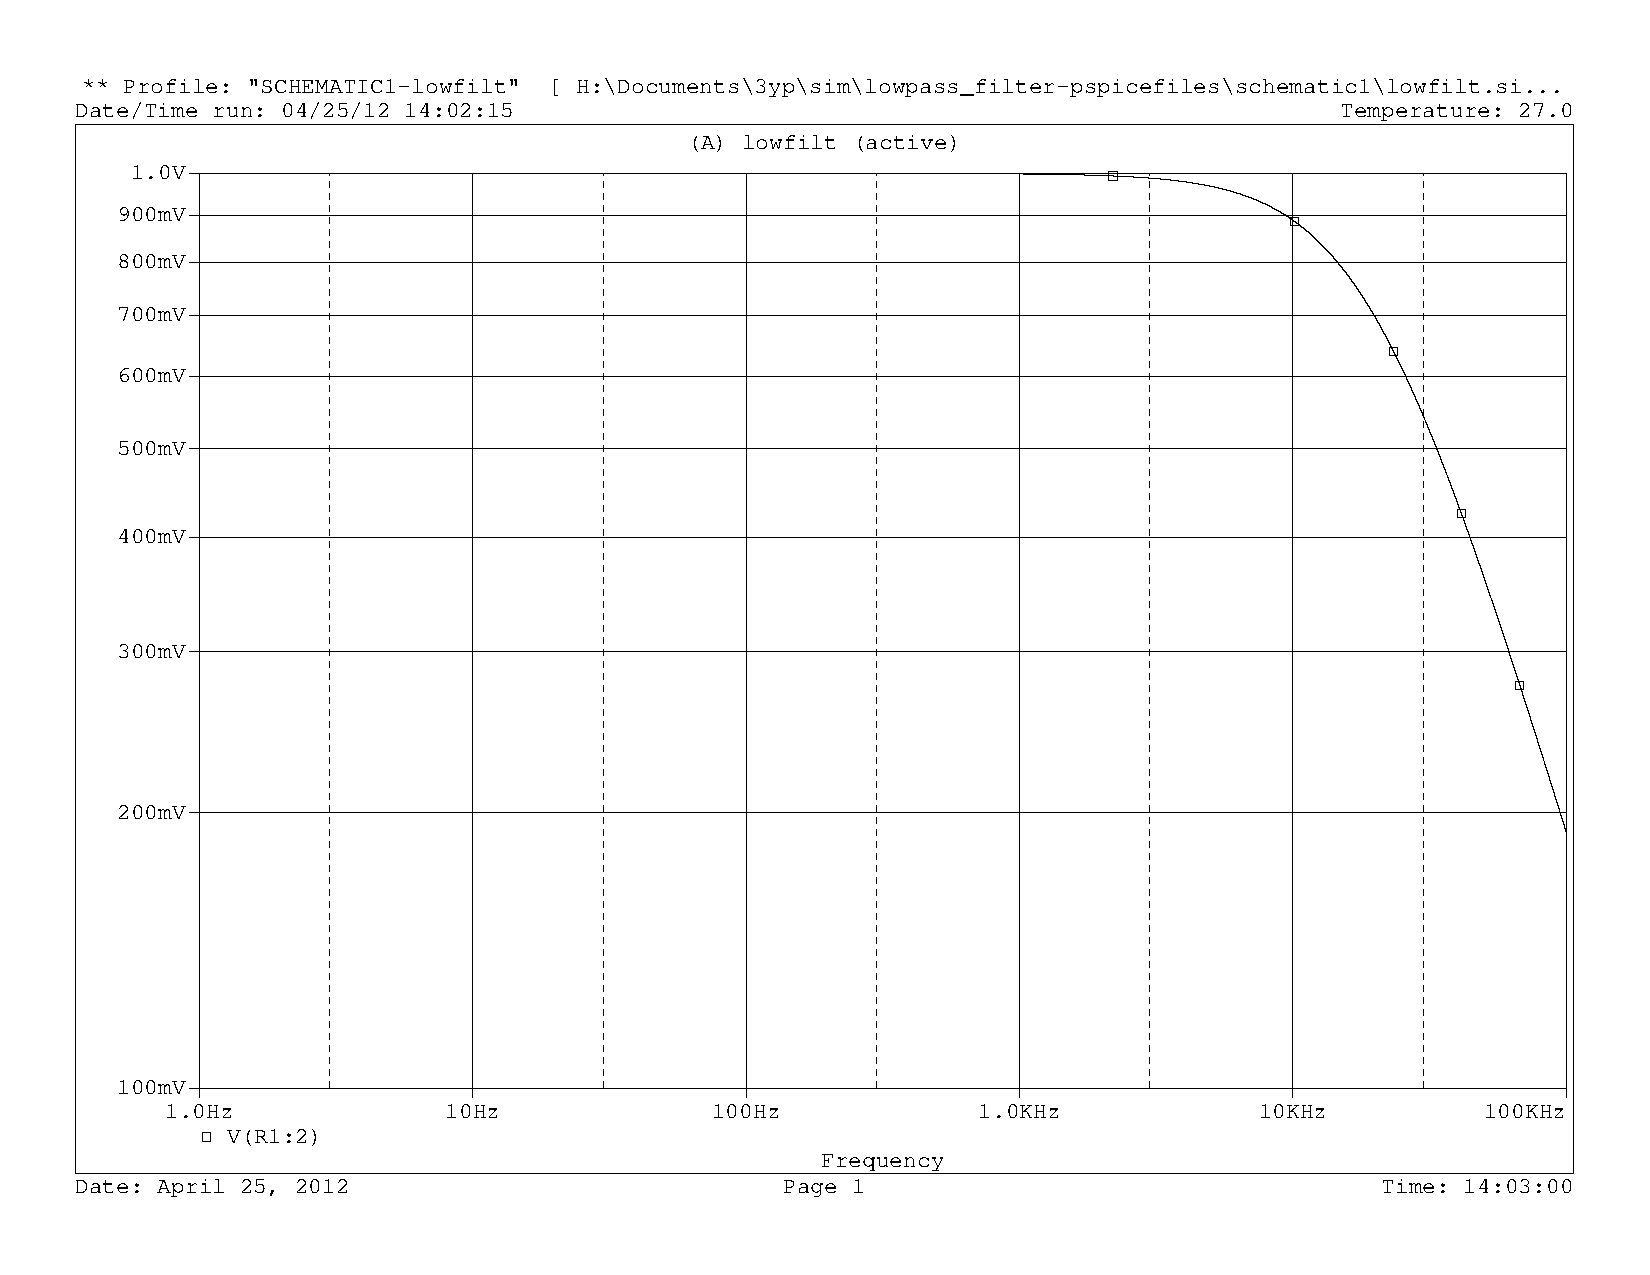
\includegraphics[width=\textwidth]{./img/signal_conditioning_sim.pdf}
	\label{fig:sigcondmodel}
	\caption{Simulation results of the signal conditioner}
\end{figure}

\subsection{Summing Amplifier}
A model of the summing amplifier was produced to check that it would function
as desired.
As the amplifier being used was not originally conceived for the use to which
it is put to in this project, modelling was even more important to check that
it would function correctly.
